% !TeX root = ../thuthesis-example.tex

\chapter{Platform development}

Several challenges were faced during development:
\begin{enumerate}
    \item Distribution of the source code;
    \item Distribution of the NUIX-Studio App demos;
    \item Creating Tutorials;
    \item Providing an API for external projects;
    \item Updating the dependencies;
    \item Rewriting the code to support new architectures.
\end{enumerate}

The platform's source code is hosted at NUIX-Studio~\cite{NUIXStudio} repository. The source code distribution required keeping the repository size at a minimum while providing an easy installation procedure. NUIX-Studio was shared as a separate package to meet these requirements.

The NUIX-Studio platform prototypes did not initially support Virtual reality (Figure~\ref{fig:Prototype2-figure}).


\begin{figure}
  \centering
  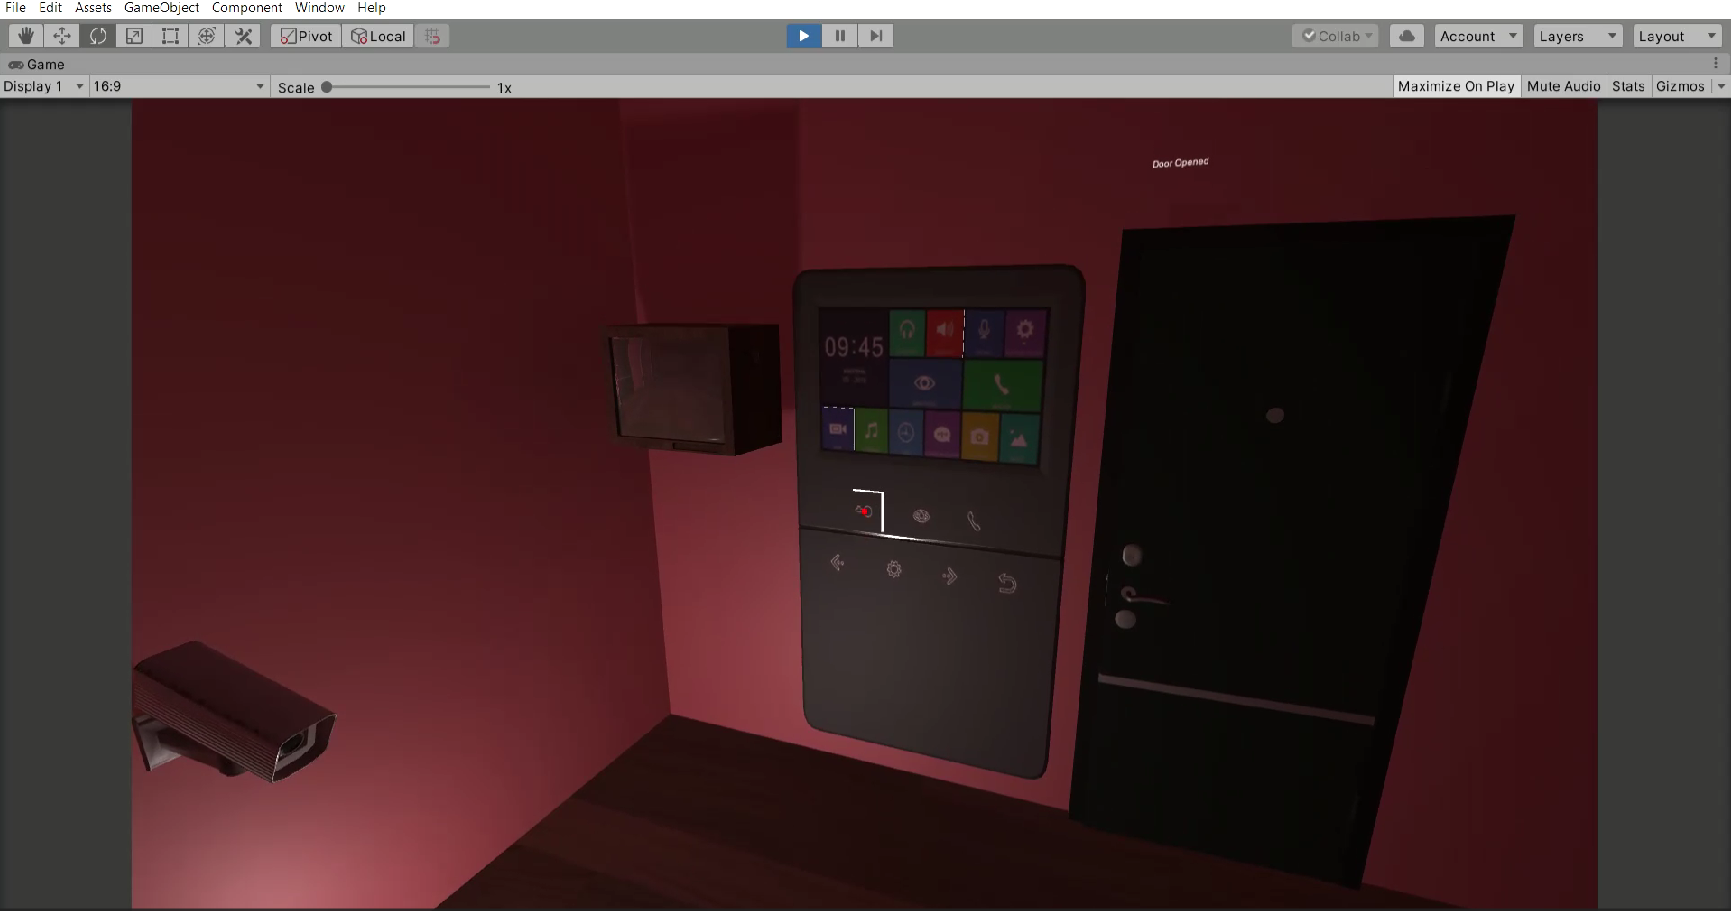
\includegraphics[width=0.9\linewidth]{figures/Prototype2.png}
  \caption{The second prototype of the VR-IoT Research platform}
  \label{fig:Prototype2-figure}
\end{figure}

The final structure used in NUIX-Studio is different from the structure in Figure~\ref{fig:Prototype3Structure-figure}. The server was responsible for storing and synchronizing item parameters and maintaining all the Unity-specific functionality of the previous prototypes. The Unity Integration package's job was to create Item representations for Virtual reality and share them to other NUIX-Studio App instances as Unity objects. This approach's main limitation is that Unity objects have a much bigger size than the Data Transfer Objects (DTO) used in the final prototype. These Unity objects were synchronized for every frame of the simultaneous work, which dramatically reduced the NUIX-Studio App instances' performance and made the solution not scalable.

\begin{figure}
  \centering
  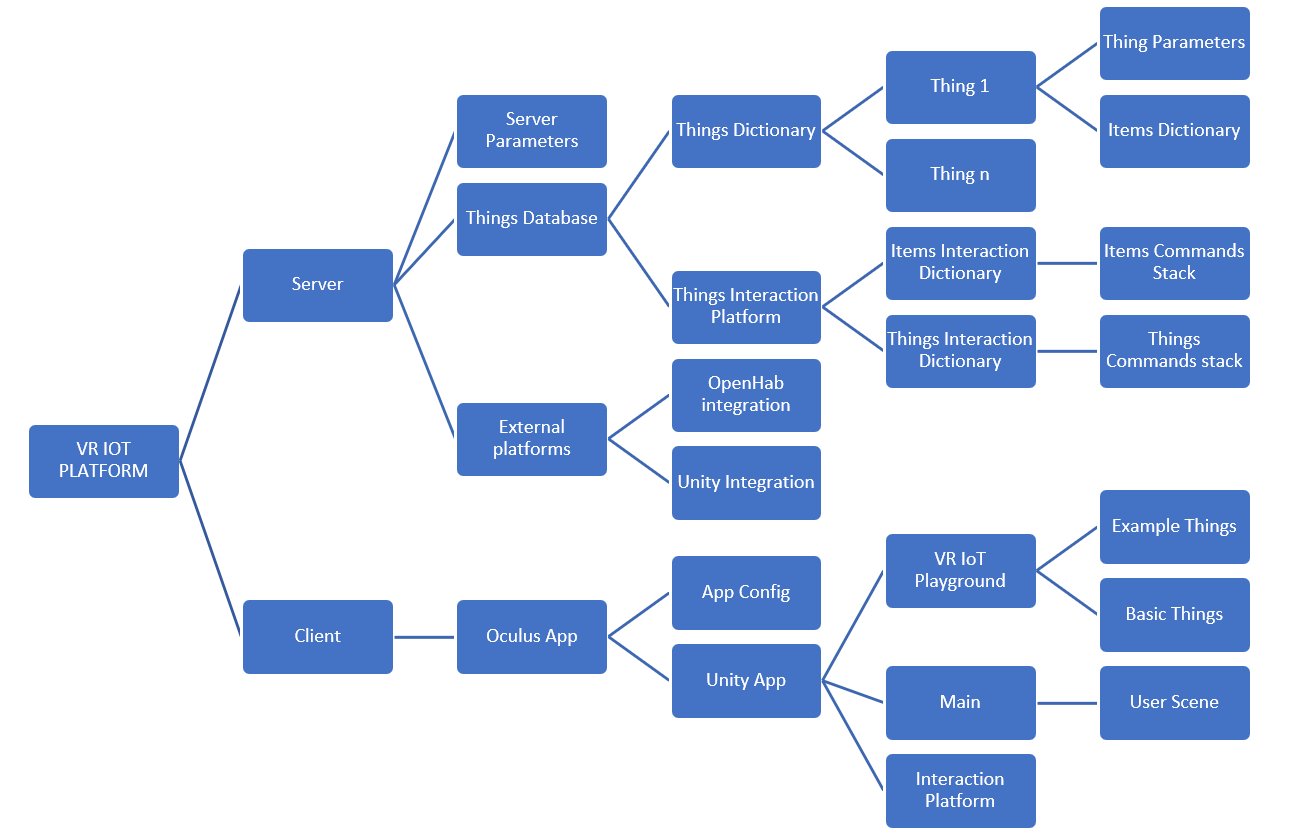
\includegraphics[width=0.9\linewidth]{figures/Prototype3Structure.png}
  \caption{The third prototype's structure}
  \label{fig:Prototype3Structure-figure}
\end{figure}

The third prototype provided only a button Widget (Figure~\ref{fig:Prototype3-figure}), but after integrating the Mixed Reality Toolkit into the fourth prototype (Figure~\ref{fig:Prototype4-figure}), additional Widgets were added to the platform. In the fourth prototype, a virtual copy of the real-world Smart home environment was used with virtual items added, such as location, contact, player, switch, and dimmer. Also, several Widgets were supported: sight sensor, motor, light widget, pressure sensor, video streaming screens, and gesture recognition.

\begin{figure}
  \centering
  \subcaptionbox{The third prototype of the VR-IoT Research platform. Button Widget.\label{fig:Prototype3-figure}}
    {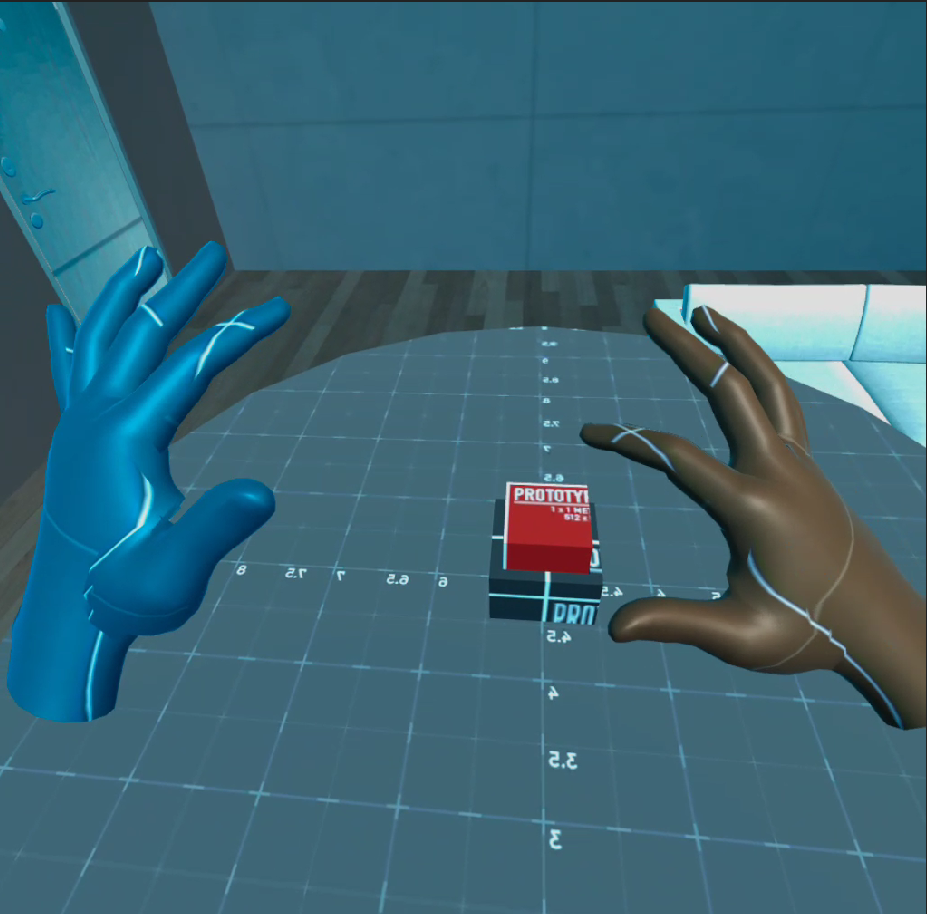
\includegraphics[width=0.435\linewidth]{figures/Prototype3.png}}
  \subcaptionbox{The fourth prototype of the VR-IoT Research platform.\label{fig:Prototype4-figure}}
    {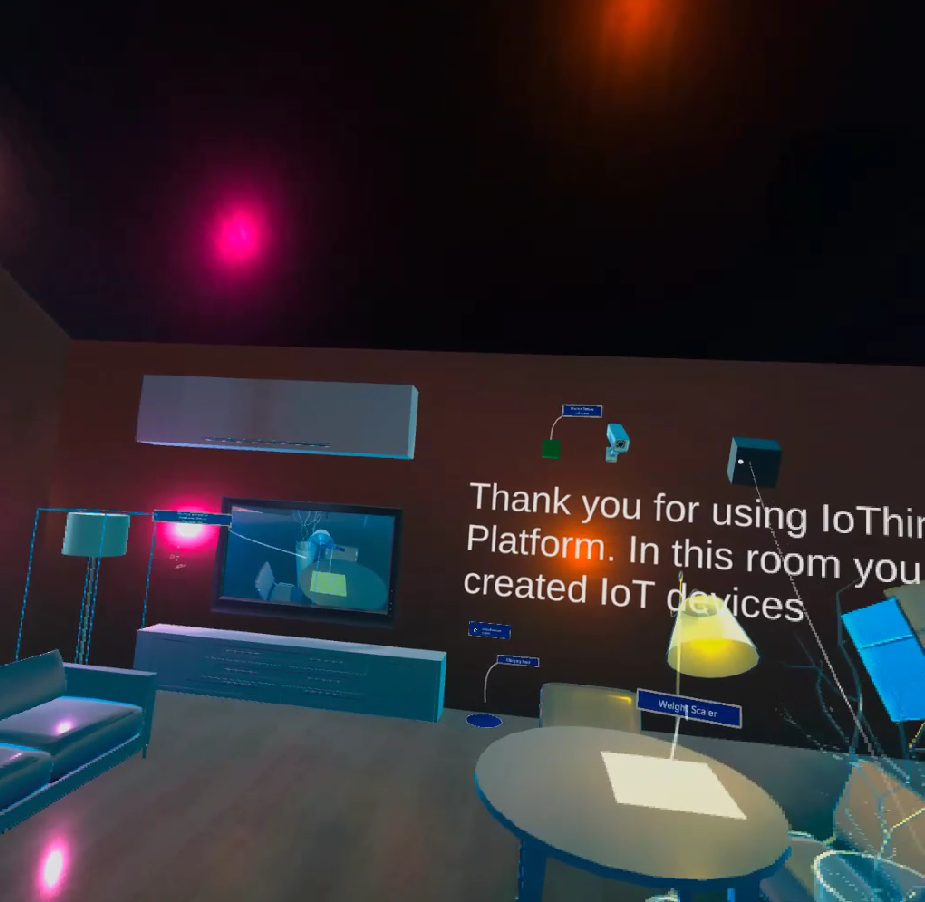
\includegraphics[width=0.44\linewidth]{figures/Prototype4.png}}
  \caption{Prototypes of the UNIX-Studio App.}
  \label{fig:NUIXStudioPrototypes-figure}
\end{figure}

Another important feature added in the fourth prototype was the Input Simulation Service (Figure~\ref{fig:InputSimulation-figure}). In most previous cases, testing the interaction with Widgets required using a Virtual Reality Headset. To use an Oculus Quest VR Headset, developers need to prepare their workplace. Firstly, the environment for using the Virtual Reality Headset must be well lit, otherwise, the Virtual Reality Headset's position detection in the world space will not work correctly. Secondly, the developer must have sufficient amount of space around him to be able to move his Virtual Reality Headset controllers or hands freely. Unfortunately, these requirements for setting up the environment are often infeasible. With the help of the Input Simulation Service system, based on the Mixed Reality Toolkit, it became possible not only to move inside the virtual world but also to make movements with virtual hands, including simulating the various gestures.

\begin{figure}
  \centering
  \subcaptionbox{Pinching gesture simulation\label{fig:InputSimulation-a}}
    {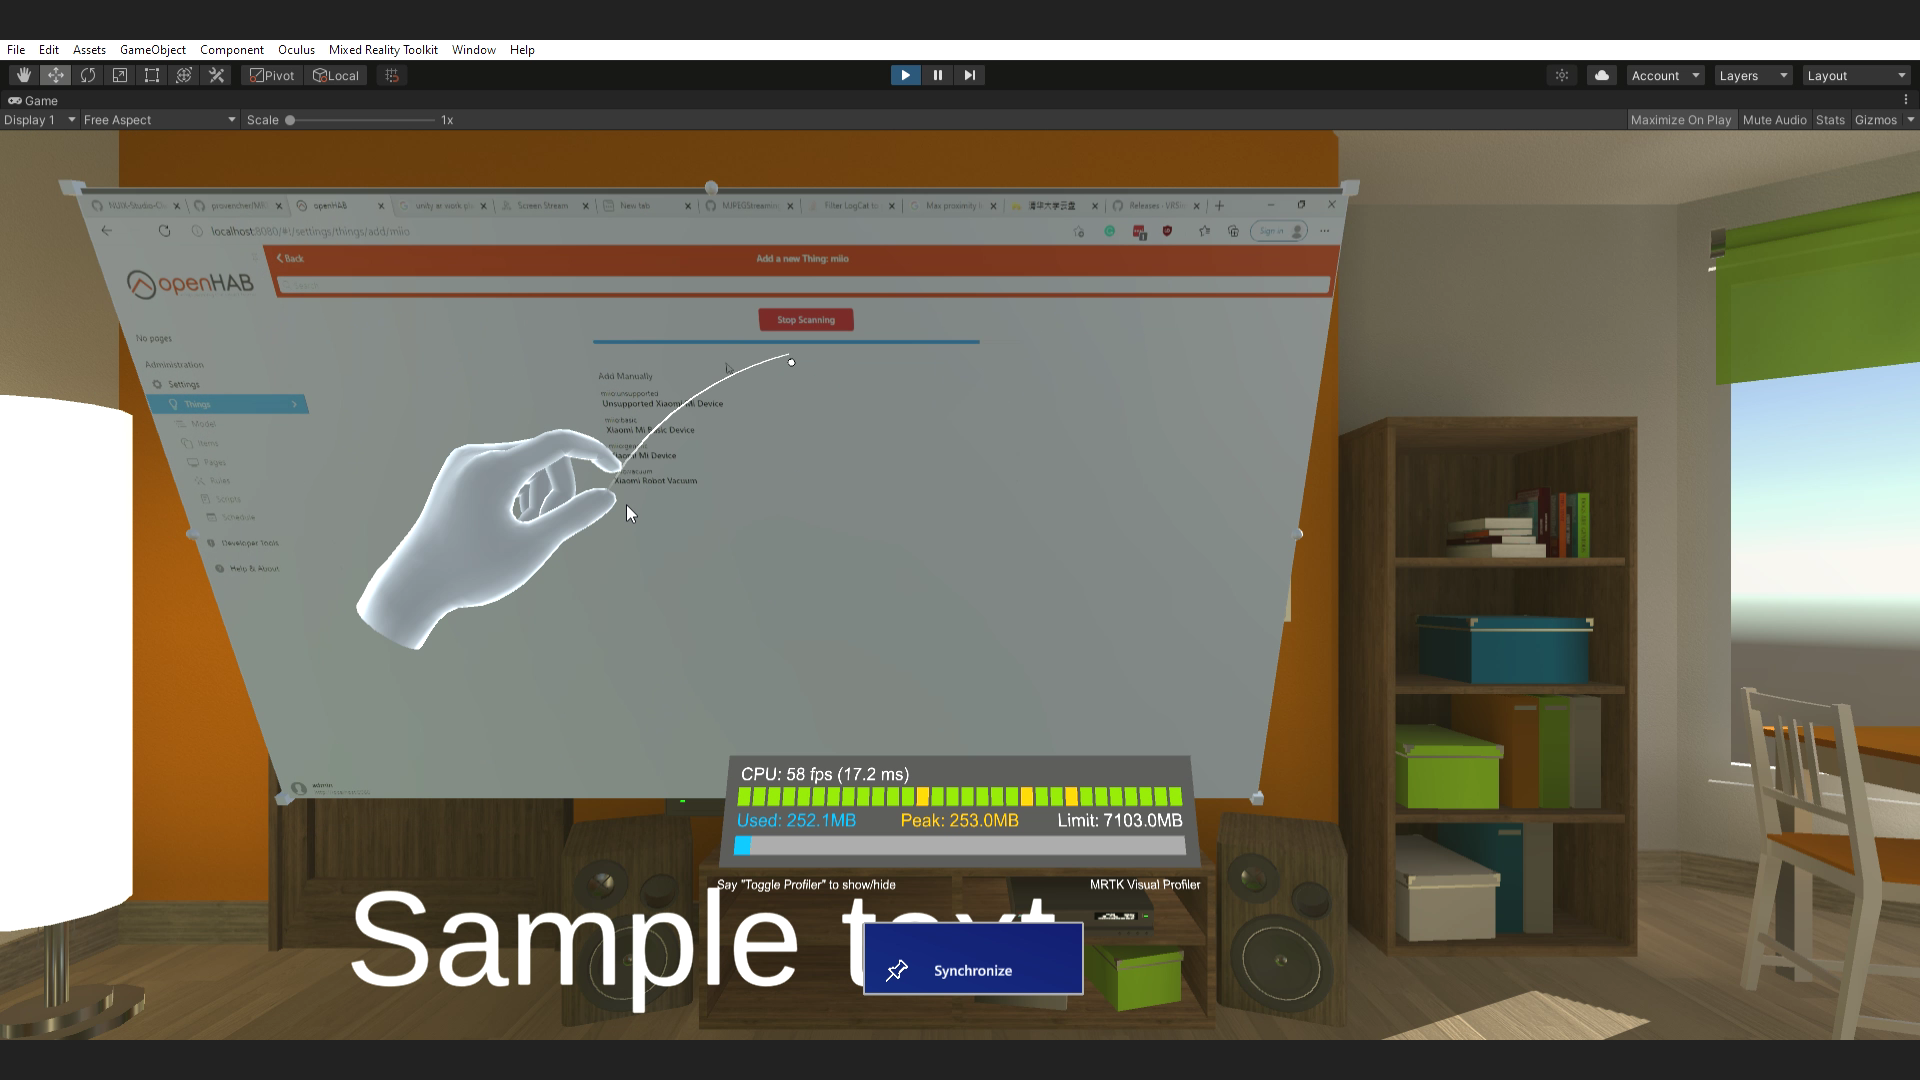
\includegraphics[width=0.45\linewidth]{figures/InputSimulation1.png}}
  \subcaptionbox{Pointing Gesture simulation\label{fig:InputSimulation-b}}
    {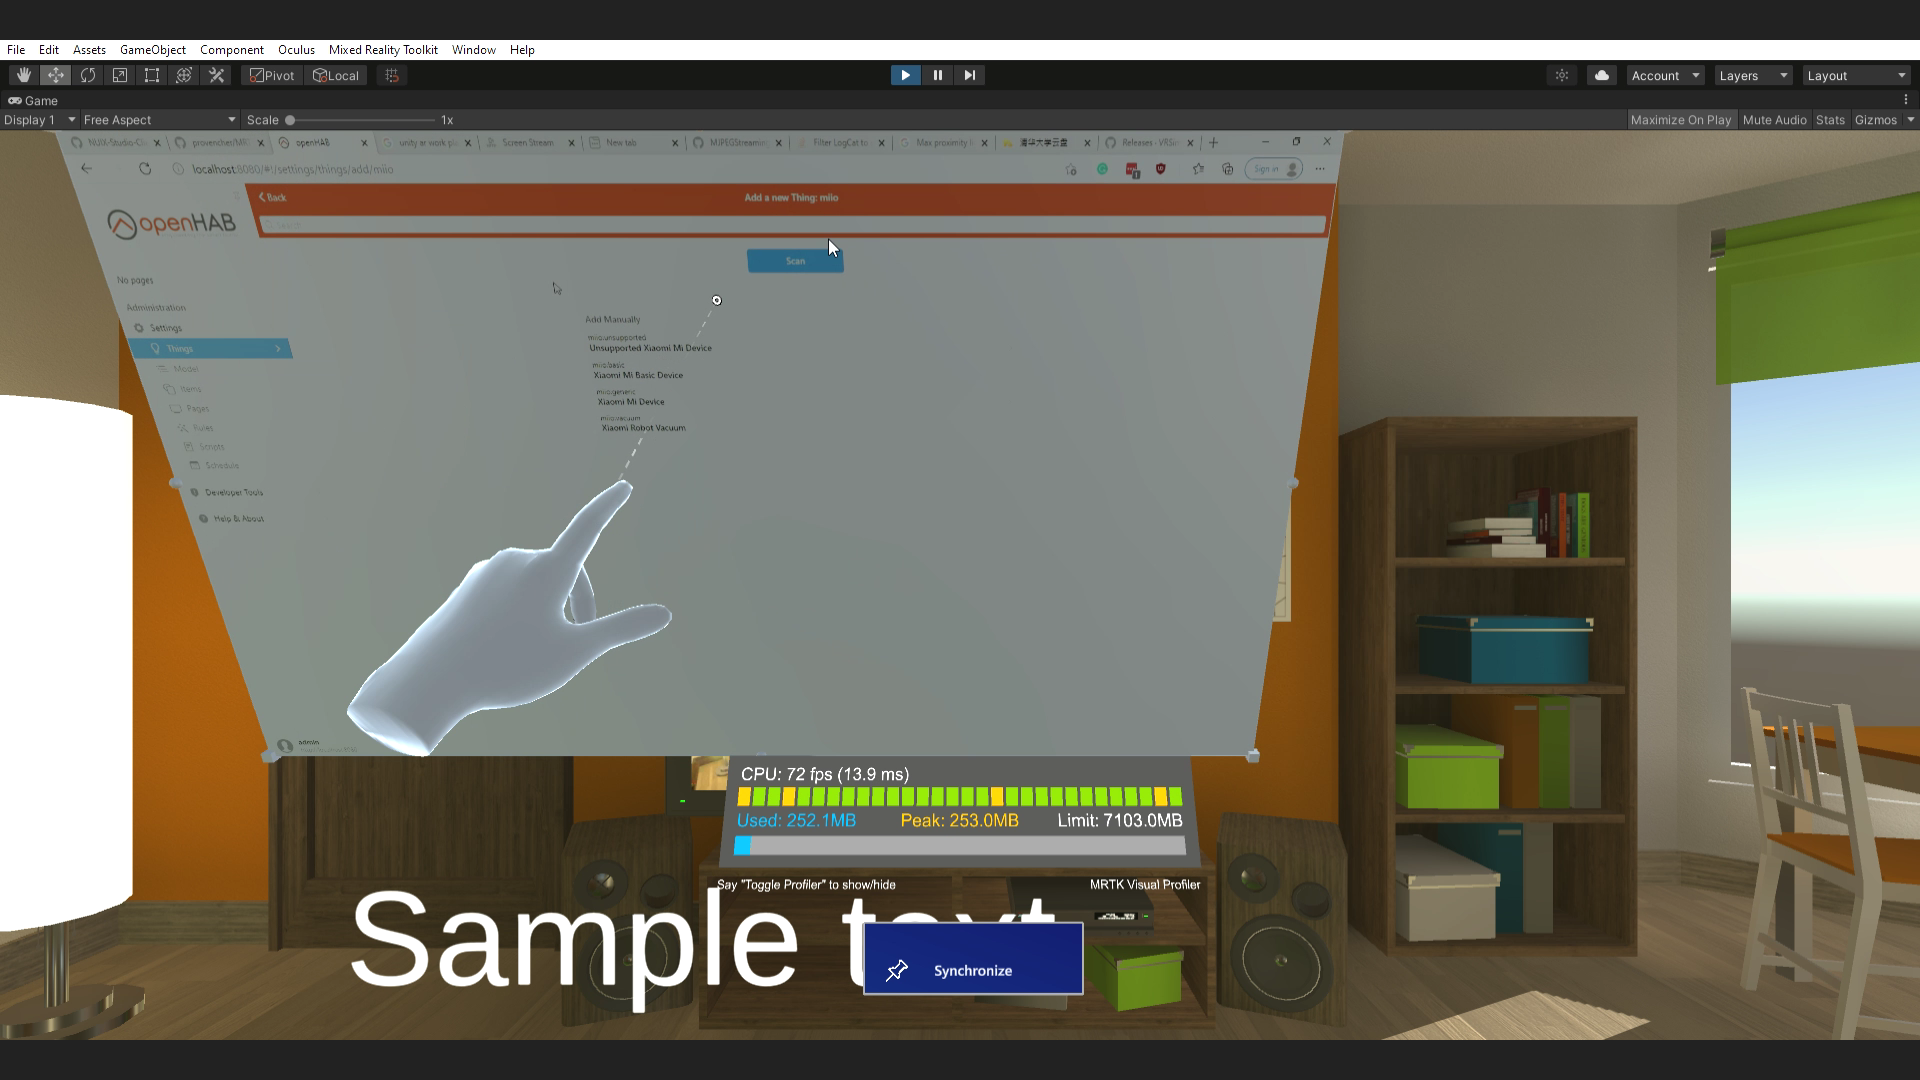
\includegraphics[width=0.45\linewidth]{figures/InputSimulation2.png}}
  \caption{Simulations of gestures on the UNIX-Studio App running on a PC.}
  \label{fig:InputSimulation-figure}
\end{figure}

In the final prototype (Figure~\ref{fig:FinalPrototypes-figure}), the code for most of the items has been rewritten to support the new architecture defined in the previous chapters. 

The other changes in the fifth prototype are:
\begin{enumerate}
    \item Performance improvements. By optimizing rendering for Oculus Quest, the framerate in the same scene (Smart home environment) has increased from 30 to over 72 frames per second;
    \item Updated dependencies. Mixed reality toolkit new features support has been added;
    \item Simplified installation. Packages for integration of Oculus and Mixed Reality toolkit have been added to the main project;
    \item Extended documentation. Each Widget's functionality has been summarized. Researchers got better explanation of how to create their own Widgets.
\end{enumerate}


\begin{figure}
  \centering
  \subcaptionbox{Typing on the virtual keyboard. \label{fig:FinalPrototype-figure}}
    {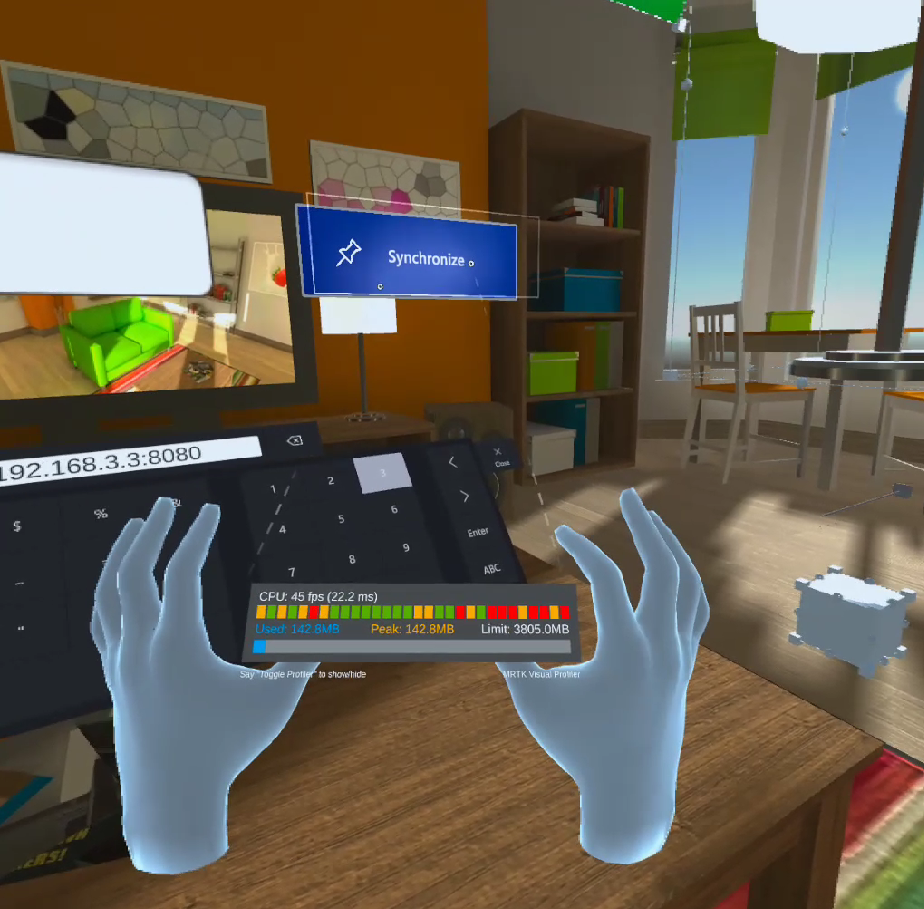
\includegraphics[width=0.45\linewidth]{figures/FinalPrototype.png}}
  \subcaptionbox{Virtual smartphone streaming image from the real smartphone.\label{fig:Prototype5-figure}}
    {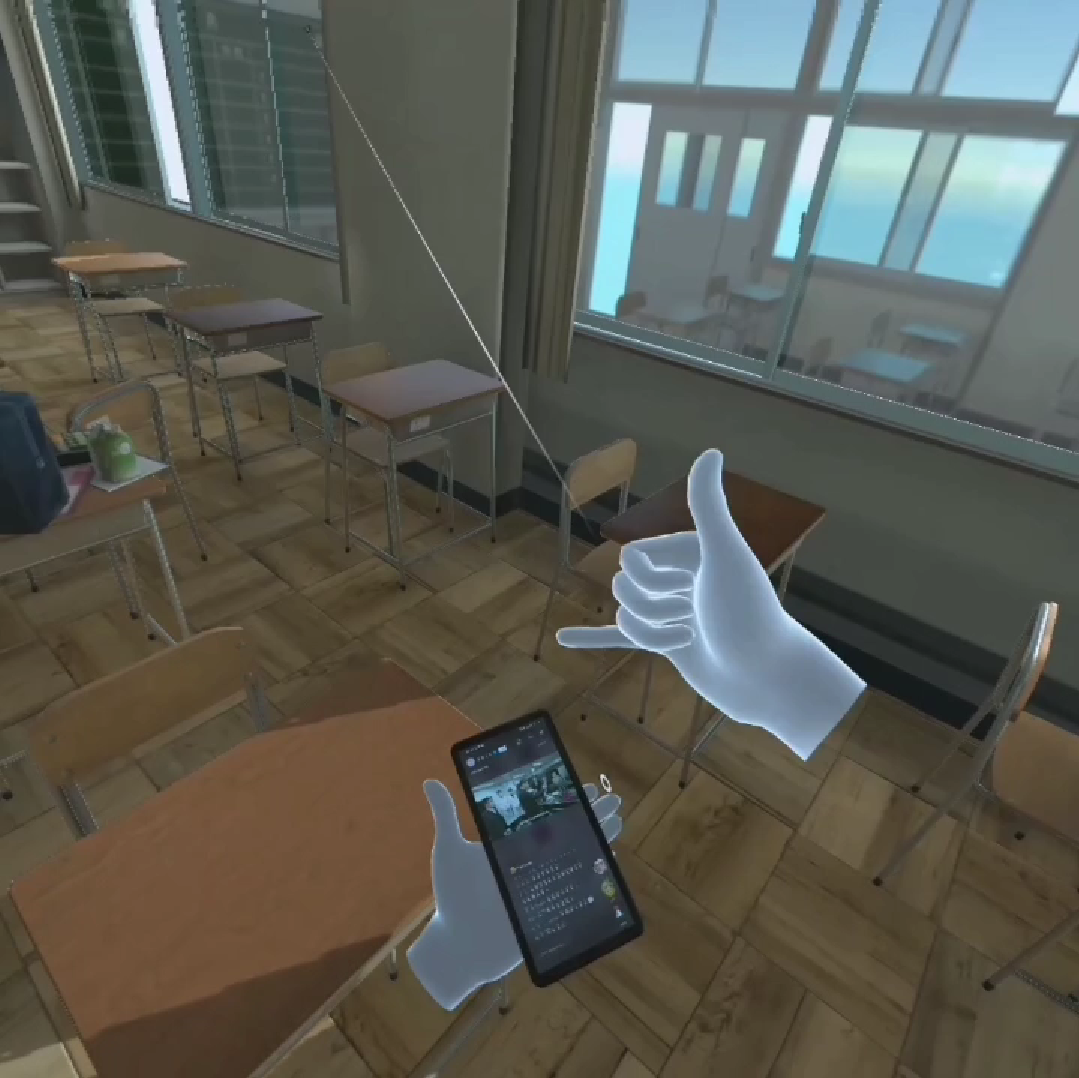
\includegraphics[width=0.45\linewidth]{figures/Prototype5.png}}
  \caption{Screenshots of the final prototypes of the NUIX-Studio App.}
  \label{fig:FinalPrototypes-figure}
\end{figure}